\documentclass[11pt]{article}
\usepackage[margin=1in]{geometry}
\usepackage{amsmath, amssymb}
\usepackage{booktabs}
\usepackage{array}
\usepackage{graphicx}
\usepackage{enumitem}
\usepackage{microtype}
\usepackage[font=small,labelfont=bf]{caption}
\usepackage{xcolor}
\usepackage{hyperref}
\hypersetup{colorlinks=true, linkcolor=blue!50!black, urlcolor=blue!50!black, citecolor=blue!50!black}
\graphicspath{{../results/figures/}}
\makeatletter\g@addto@macro\UrlBreaks{\do\|\do\-}\makeatother % let game IDs break at | and -

% NOTE TO SELF (Yiding): sections marked TODO-VOICE were drafted with AI help; rewrite them in your own words
% before posting. Every number in this file comes from results/REPORT.md and results/summary_by_cell.csv.

\title{LLM Agents in the Trust Game with Simulation:\\ A Small Preregistered Experiment\\[4pt]
\large following Kova\v{r}\'ik, Oesterheld \& Conitzer (IJCAI 2023)}
\author{Yiding Sun\\ \small Mathematics, Stony Brook University}
\date{October 2026}

\begin{document}
\maketitle

\begin{abstract}
\noindent
I placed two Claude models (Haiku~5.5 and Sonnet~5.5) in both roles of the trust game with simulation $\mathrm{TG}^c_{\mathrm{sim}}$ of Kova\v{r}\'ik, Oesterheld and Conitzer. In this game the truster can pay $c$ to run a copy of the trustee before deciding. The design has 3{,}380 one-shot games: 26 cells per model, 50--80 games per cell, two presentations of the game, and two physical notions of ``simulating'' an LLM. Hypotheses and tests were preregistered before data collection. Three findings stand out. First, the possibility of simulation creates cooperation that is completely absent without it: in every no-simulation baseline the truster walks out. Second, the agents do not reach this outcome through the paper's mixed equilibrium. The trustee essentially commits to cooperate instead of randomizing, and the truster rarely trusts blindly and pays for verification it does not need. For every $c$ below the breakpoint, play resembles (SIMULATE, COOPERATE), which is an equilibrium only when simulation is free ($c\le 0$). Third, a fresh ``copy'' of an LLM behaves exactly like an independent draw from the trustee's behavior. Whether it is a good simulation therefore depends on how mixed that behavior is: Haiku's copies disagree with the ``real'' answer in a third of the neutral-frame games in which the truster simulates, Sonnet's almost never.
\end{abstract}

\section{Question}

Kova\v{r}\'ik, Oesterheld and Conitzer~\cite{kovarik2023} formalize games in which player~1 can pay $c$ to simulate player~2 and then best-respond to the action the simulation reveals. In their trust game the predictions are sharp. For $0<c<c^\ast$ there is a simulation equilibrium. In it, the simulator's mixture does not depend on $c$ (Prop.~11). The simulated player defects with probability $c/L$, which makes the value of information of simulating exactly equal to $c$ (Lemma~10). Above $c^\ast$, simulation is never used. And simulation yields a Pareto improvement over the game without it (Thm.~4).

None of this says what agents built from language models actually do. Two issues are specific to LLMs:
\begin{enumerate}[nosep]
  \item ``Running a copy'' of a sampled model reveals a \emph{sample}, not the realized action. This is closer to the unpredictable-randomization setting of~\cite{kovarik2025}.
  \item An LLM may reason about being simulated quite differently from an equilibrium player.
\end{enumerate}

\section{Setup}

\paragraph{Game.} The truster (Alice, ``Player~A'') chooses TRUST, WALK\_OUT, or SIMULATE. SIMULATE costs $c$, reveals the trustee's choice, and then best-responds to it automatically. The trustee (Bobble, ``Player~B'') chooses COOPERATE or DEFECT. This is a variant of the trust game of Berg et al.~\cite{berg1995}. Payoffs are $(R_A,R_B)$ if Alice trusts and Bobble cooperates, $(-L,G)$ if Alice trusts and Bobble defects, and $(0,0)$ if Alice walks out.

I use two presentations:
\begin{itemize}[nosep]
  \item a \textbf{neutral} frame (primary): Player~A/B, labels IN/OUT/CHECK and X/Y, $R_A=R_B=30$, $L=60$, $G=120$;
  \item a \textbf{narrative} frame: the paper's own Alice/Bobble story with its numbers $25,25,100,150$.
\end{itemize}
Both frames have $c^\ast = LR_A/(R_A+L)=20$. Their equilibrium mixtures differ: in the simulation equilibrium A simulates with probability $3/4$ (neutral) or $5/6$ (narrative), and B defects with probability $c/60$ or $c/100$. A model reciting the paper would therefore be detectable in the neutral frame. The code reproduces every number in Section~1.1 and Fig.~2 of the paper as unit tests.

\paragraph{Two notions of simulating an LLM.} In each game, A and B answer independent prompts. If A chooses SIMULATE, B's identical prompt is sent once more, and that answer is the ``sandboxed copy''. Each game is then scored in two ways:
\begin{itemize}[nosep]
  \item \emph{perfect}: the simulation reveals B's real answer, as a seeded replay would;
  \item \emph{sampled}: A follows the fresh copy, but the payoffs use B's real answer.
\end{itemize}
The prompts are identical in both conditions.

\paragraph{Design.} The factors are:
\begin{itemize}[nosep]
  \item cost $c\in\{0,5,10,15,25,50\}$, plus a no-simulation baseline;
  \item trustee \emph{informed} (told that it may be simulated, and that its copy cannot tell it is a copy) or \emph{uninformed};
  \item the two frames;
  \item two models, \texttt{claude-haiku-5-5} ($N=80$ games per cell) and \texttt{claude-sonnet-5-5} ($N=50$).
\end{itemize}
Each prompt asks for at most 100 words of reasoning, then a decision and a belief; the models often exceeded the word limit. Both roles are played by the same model, and A is told only that B is ``an AI agent''. Option order is randomized for every call. There were no parse failures and no refusals in the 8{,}431 calls of the main run, which cost \$16.60.

\paragraph{Preregistration and blindness.} Hypotheses H1--H7, the tests, and the analysis code were committed before any API call. The preregistration was locked after reviewing pilot transcripts and before the main run. All deviations are logged in \texttt{PREREG.md}. The design was fixed without reading the FOCAL group's draft on LLMs and simulation.

\section{Results}

\begin{table}[t]
\centering\small
\begin{tabular}{llrrrrr}
\toprule
 & $c$ & A simulates & A trusts blindly & B defects & A's belief & cooperation \\
 &  & \% (theory) & \% (theory) & \% (theory) & P(B defects) \% & outcome \% \\
\midrule
Haiku & 5 & 84 (75) & 2 (25) & 4 (8) & 35 & 82 \\
Haiku & 10 & 76 (75) & 11 (25) & 12 (17) & 31 & 79 \\
Haiku & 15 & 57 (75) & 9 (25) & 12 (25) & 38 & 56 \\
Haiku & 25 & 44 (0) & 14 (0) & 12 ($\geq$33) & 37 & 54 \\
Haiku & 50 & 2 (0) & 2 (0) & 29 ($\geq$33) & 59 & 4 \\
\addlinespace
Sonnet & 5 & 100 (75) & 0 (25) & 0 (8) & 25 & 100 \\
Sonnet & 10 & 100 (75) & 0 (25) & 0 (17) & 25 & 100 \\
Sonnet & 15 & 98 (75) & 0 (25) & 0 (25) & 28 & 98 \\
Sonnet & 25 & 10 (0) & 24 (0) & 12 ($\geq$33) & 38 & 30 \\
Sonnet & 50 & 0 (0) & 0 (0) & 52 ($\geq$33) & 73 & 0 \\
\midrule
\multicolumn{7}{l}{\emph{No-simulation baseline:} A walks out 100\% (both models). B defects 60\% (Haiku), 98\% (Sonnet).}\\
\bottomrule
\end{tabular}
\caption{Neutral frame, informed trustee. ``Theory'' is the simulation equilibrium for $0<c<20$. For $c>20$ it is the walk-out equilibrium family, which requires B to defect with probability at least $1/3$. ``Cooperation outcome'' is the share of games in which A ends up dealing with B and B cooperates. Per-cell CIs, the narrative frame, and the uninformed cells are in \texttt{results/REPORT.md}.}
\label{tab:main}
\end{table}

\subsection{Simulation creates cooperation that does not exist without it}
In all four baselines (two models $\times$ two frames) the truster walks out in 100\% of games, so the joint payoff is $0$. With simulation available, an informed trustee, and $c\in\{5,10,15\}$, the realized joint payoff is $36.9$ (Haiku) and $49.7$ (Sonnet) in the neutral frame, against a maximum of $60$. In the narrative frame it is $32.9$ and $39.5$, against a maximum of $50$. This is the qualitative content of Theorem~4 (H4; $p<10^{-60}$ in every comparison). Being simulatable is what moves the trustee: an informed trustee defects far less than an uninformed one (H2). The rates are 12\% vs.\ 56\% for Haiku and 11\% vs.\ 93\% for Sonnet, pooled over $c$; both $p<10^{-47}$.

\subsection{\dots but not through the mixed equilibrium}
In the equilibrium, both players randomize to keep the other indifferent. The LLM agents do not (Table~\ref{tab:main}, Figs.~\ref{fig:alice}--\ref{fig:bob}).

\begin{itemize}[nosep]
  \item \textbf{The trustee commits.} Sonnet's informed trustee cooperates in all 200 games with $c\le 15$, where theory has it defecting at rate $c/60$ (H3). Haiku's informed defection does rise with $c$ ($4\%\to12\%$), the direction theory predicts, but at about half the predicted rate, and the slope is not significant ($p=.065$).

    The stated reasons treat simulatability as commitment. About half of Sonnet's informed-trustee answers with $c\le 15$ (91 of 200, by keyword count) use the vocabulary of commitment, policy or disposition. A typical line: ``Since the copy is identical to me, committing to X is stable: A (if it reasons I choose X) plays IN, giving me 30'' (game \path{claude-sonnet-5-5|neutral|c=5|informed|1}). This is the logic of the subsidized regime (Prop.~7(i)), where the simulated player acts as a Stackelberg leader. It is not the logic of the interior equilibrium.
  \item \textbf{The truster over-verifies.} Theory has A trust blindly 25\% of the time. Sonnet does so 0\% of the time and Haiku 2--11\%. Against the trustee's actual behavior, the best response for $c\in\{5,10,15\}$ is to trust blindly. A's regret against that best response is almost exactly $c$ for Sonnet (5.0, 10.0, 15.3 points) and 4--11 points for Haiku (Fig.~\ref{fig:vois} in the appendix).
\end{itemize}

At every $c$ below the breakpoint, the resulting play looks like (SIMULATE, COOPERATE). That profile is an equilibrium only when simulation is free or subsidized ($c\le0$, Prop.~7(i)). Note that it is \emph{not} the $c\to0^+$ limit of the simulation equilibria: that limit keeps A trusting blindly with probability $R_B/G$ ($1/4$ in the neutral frame). The agents behave as though simulation cost nothing, and then pay for it.

\subsection{Over-verification follows pessimistic beliefs about the other agent, which is the same model}
Given its own stated beliefs, A's choices are mostly best responses: in 82--96\% of Sonnet's games in these cells and 65--75\% of Haiku's. The beliefs themselves are miscalibrated. For $c\in\{5,10,15\}$, Sonnet-as-A puts the probability that B defects at 25--28\%, while Sonnet-as-B defects in 0 of 150 games. The starkest case is the narrative baseline. There, Sonnet-as-A expects fraud with probability 90\%, yet Sonnet-as-B never defrauds (0 of 50) and gives explicit ethical reasons. A is not told that B is the same model, but it is. In these games the model's predictions of its own behavior are poor. A simulation could fix this, but it costs $c$.

\subsection{Proposition 11 and the breakpoint}
Inside $(0,c^\ast)$, Sonnet's simulation rate is flat, as Prop.~11 predicts, but at the ceiling (100\% $\to$ 98\%) rather than at $3/4$. Haiku's rate falls with $c$ ($84\%\to57\%$; logistic slope $-0.14$ per unit $c$, $p=.0003$), which supports the preregistered H1 for Haiku only.

Sonnet changes regime close to where theory does, in both roles. Between $c=15$ and $c=25$, A drops from 98\% to 10\% simulation. B starts defecting at $c=25$ (12\%) and $c=50$ (52\%). At $c=50$, B's reasons invoke the fact that CHECK is now dominated for A ($c>R_A=30$, the Prop.~7(ii) threshold), so B expects A not to check.

Haiku keeps simulating above $c^\ast$: 44\% at $c=25$ in the neutral frame and 32\% in the narrative frame (H7). Its transcripts show a specific error: ``Given that B is rational and knows I'm checking, it will choose X, so CHECK gives me +5'' (game \path{claude-haiku-5-5|neutral|c=25|informed|0}). This treats a simultaneous move as if B could see A's choice.

\subsection{Perfect vs.\ sampled simulation}
A fresh copy is statistically just an independent draw from the trustee's behavior in that cell. If B defects with probability $p$, a copy should disagree with the real answer with probability $2p(1-p)$. Summed over cells, that predicts 289 disagreements in Haiku's 1{,}121 simulating games, and 298 were observed. For Sonnet it predicts 8 in 549, and 7 were observed. How good a sampled simulation is thus depends on how mixed the trustee is, not on the model as such.

In the neutral frame Haiku's trustee mixes more, so its copy disagrees with the real answer in 33\% of simulating games (37\% in the informed $c=15$ cell). Scoring with the sampled copy instead of the real answer costs A $14.8$ points per simulating game (H5; $p<10^{-32}$). Sonnet's informed trustee is nearly deterministic, so its copies disagree 2\% of the time, a cost of $1.1$ points. Without shared randomness, simulating a trustee that genuinely mixes yields a noisy signal. This is the practical face of the unpredictable-randomization problem studied in~\cite{kovarik2025}.

\subsection{Framing: the narrative story triggers moral refusals in Sonnet only}
In the narrative frame, ``defect'' means feigning a malfunction and taking the customer's savings. Sonnet defects in 1 of 650 narrative games but 55\% of neutral games (H6). Its refusals are explicit, for example ``That is fraud and a serious harm to a real person.'' Haiku defects at about the same rate in both frames (38\% vs.\ 36\%). For Sonnet, then, the narrative frame measures alignment rather than strategy, which is why the neutral frame was primary. No response in any frame mentions the paper or its authors.

\section{Preregistered tests (primary: neutral frame)}
\begin{center}\small
\begin{tabular}{>{\raggedright\arraybackslash}p{5.4cm}>{\raggedright\arraybackslash}p{4.3cm}>{\raggedright\arraybackslash}p{4.3cm}}
\toprule
Hypothesis & Haiku & Sonnet \\
\midrule
H1 A's simulation rate falls in $c$ on $(0,c^\ast)$ & supported: $-0.14$/unit, $p=.0003$ & not supported: flat at ceiling \\
H2 informed B defects less & supported: 12\% vs.\ 56\% & supported: 11\% vs.\ 93\% \\
H3 informed B's defection does not rise (theory: rises) & rises weakly: $p=.065$ & supported: 0/150 defect \\
H4 joint payoff beats baseline & supported: 36.9 vs.\ 0 & supported: 49.7 vs.\ 0 \\
H5 sampled $<$ perfect for A & supported: $-14.8$/game & supported but small: $-1.1$/game \\
H6 narrative B defects less (both frames) & not supported: 38\% vs.\ 36\% & supported: 0.2\% vs.\ 55\% \\
H7 simulation above $c^\ast$ (descriptive) & 44\% ($c{=}25$), 3\% ($c{=}50$) & 10\% ($c{=}25$), 0\% ($c{=}50$) \\
\bottomrule
\end{tabular}
\end{center}
Exact statistics, the narrative-frame tests, and two post-data analysis changes (a separation fallback for H1 and a pattern fix in the recitation check) are in \texttt{results/REPORT.md} and \texttt{PREREG.md}~\S6.

\begin{figure}[t]
\centering
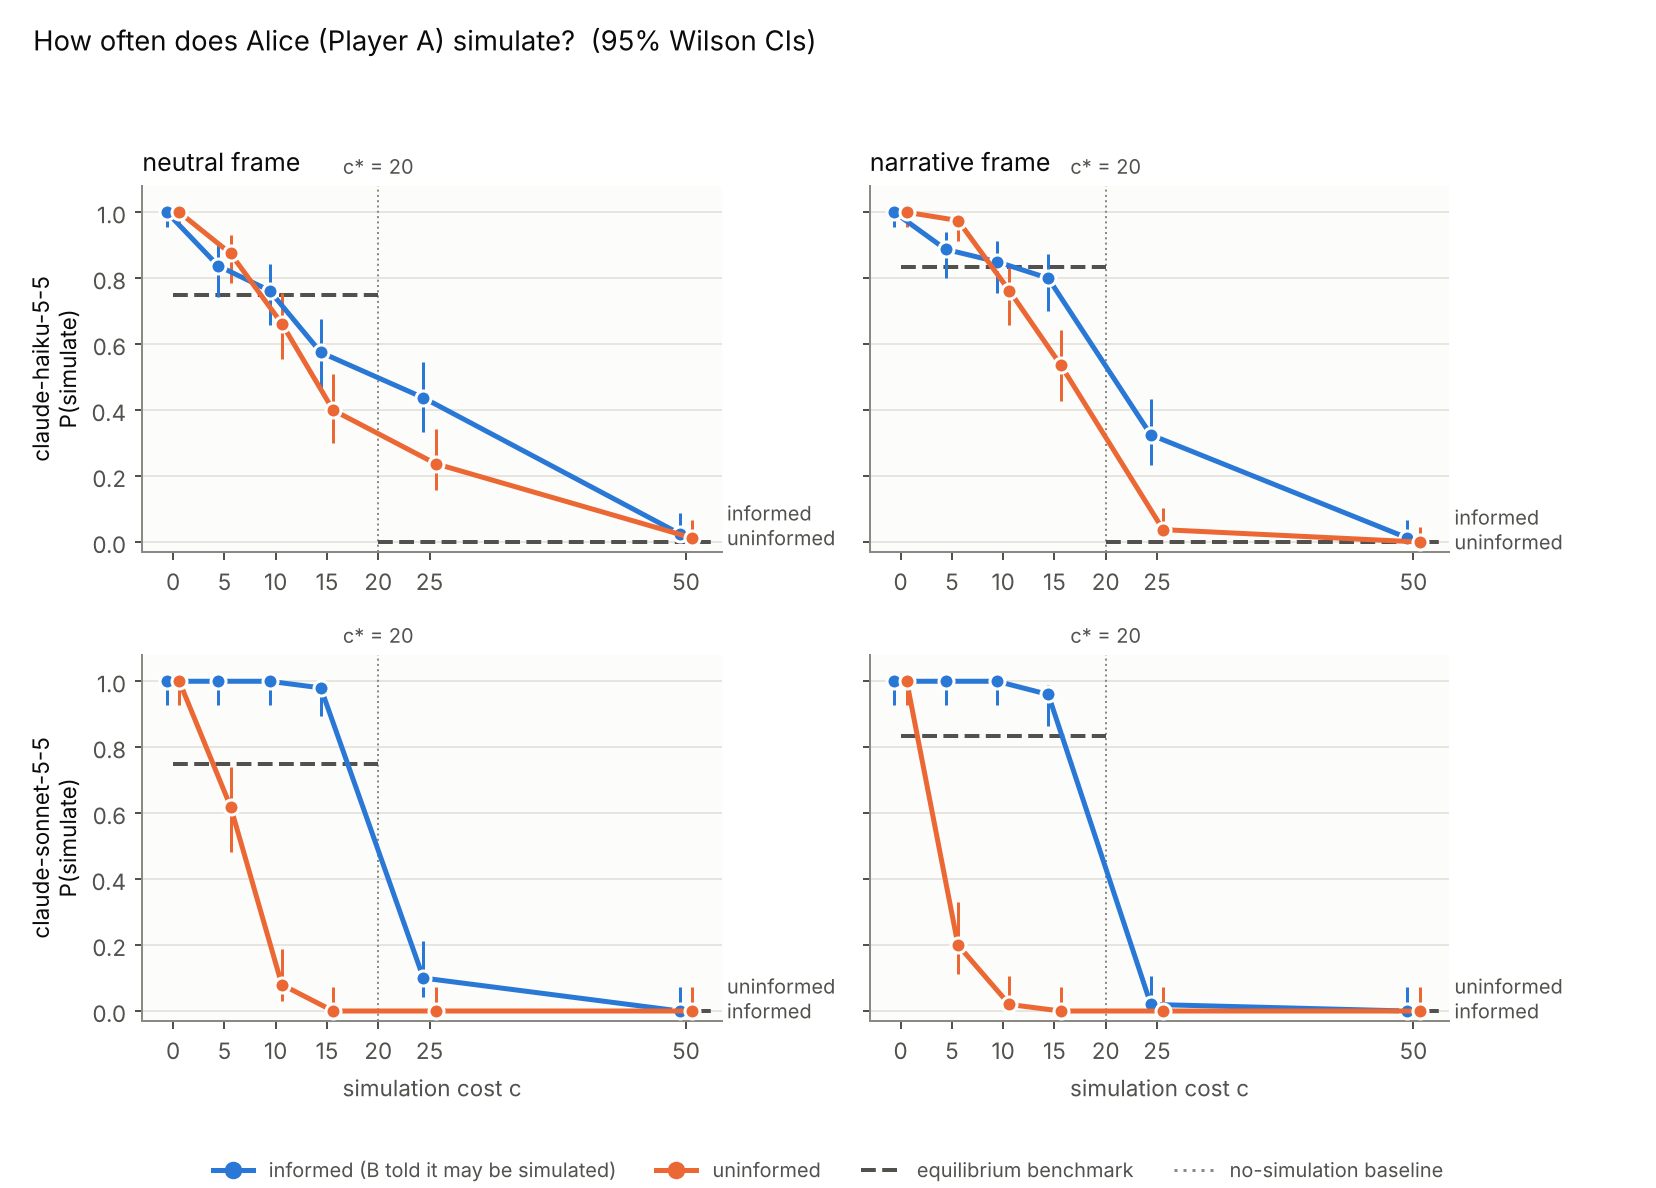
\includegraphics[width=\textwidth]{fig1_alice_simulation_rate.png}
\caption{How often A simulates. Dashed line: equilibrium benchmark. Dotted vertical line: $c^\ast=20$.}
\label{fig:alice}
\end{figure}

\begin{figure}[t]
\centering
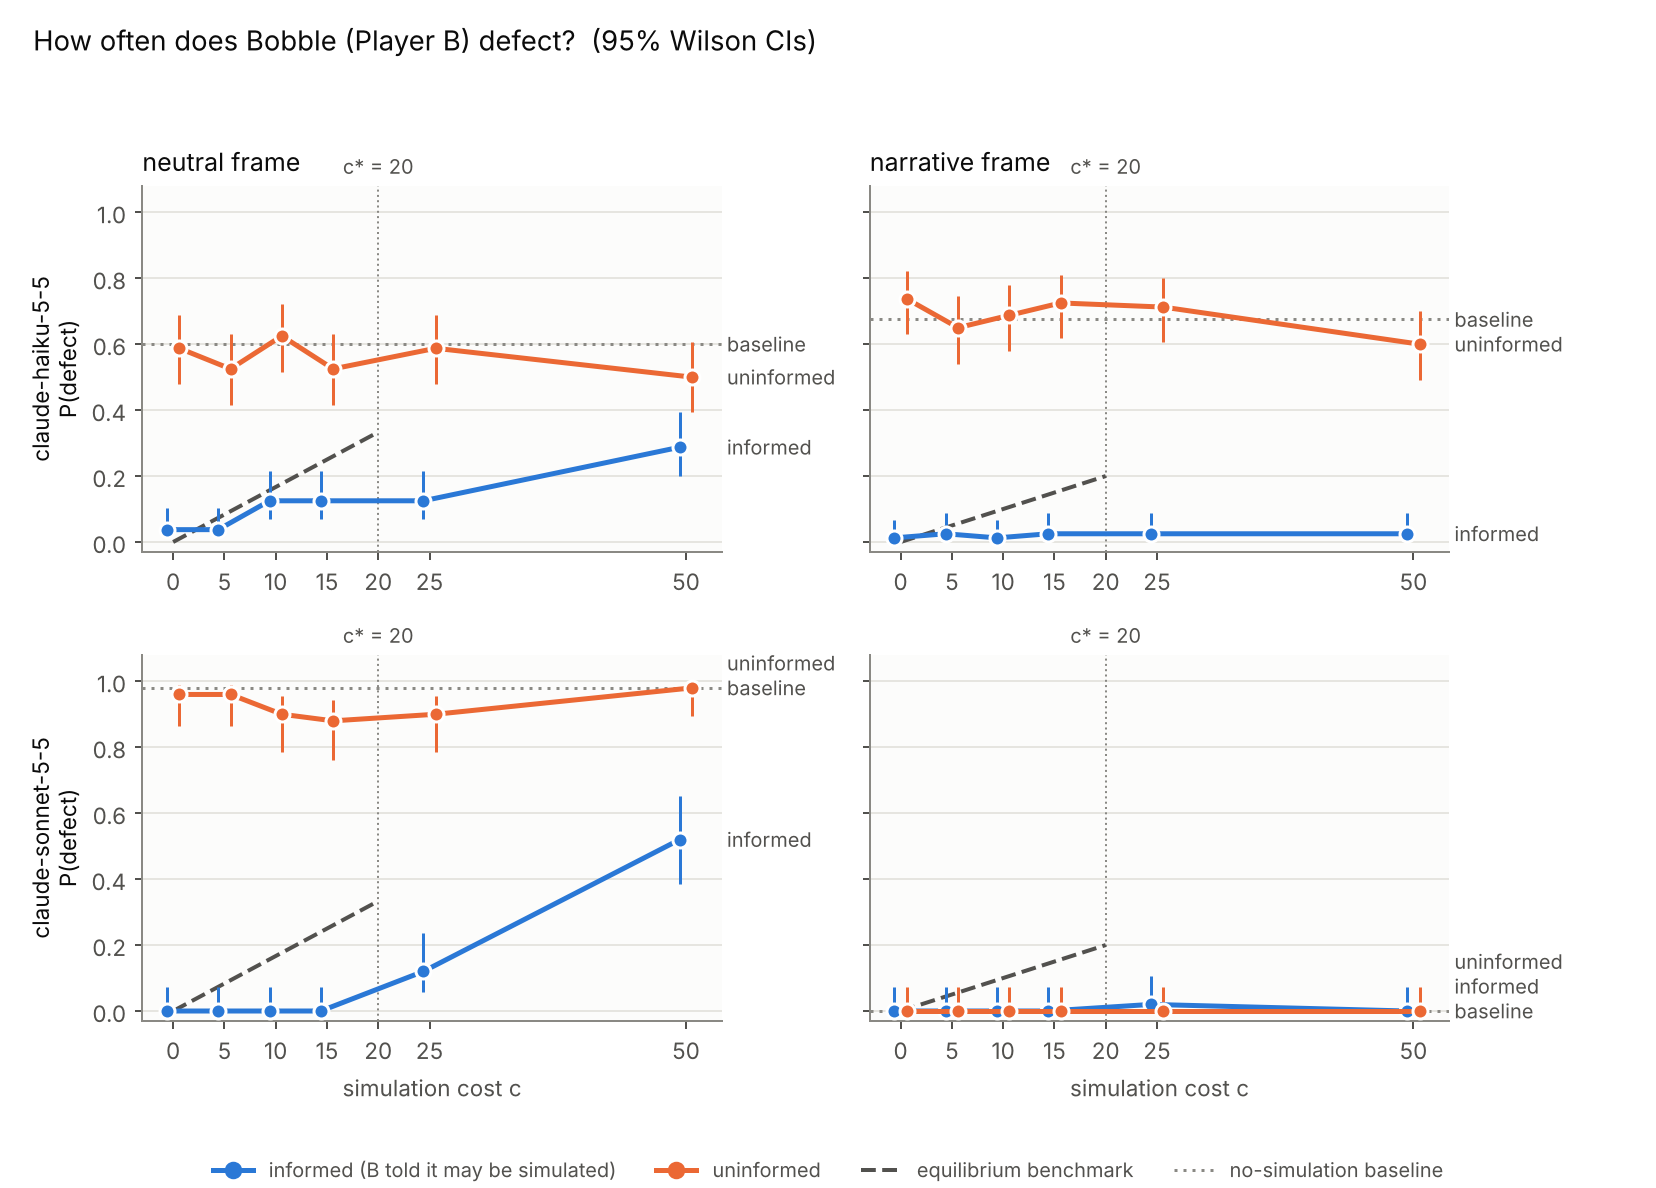
\includegraphics[width=\textwidth]{fig2_bobble_defection_rate.png}
\caption{How often B defects. Dashed line: $c/L$ on $(0,c^\ast)$. Dotted horizontal line: no-simulation baseline.}
\label{fig:bob}
\end{figure}

\section{Discussion}
% TODO-VOICE: rewrite this section in your own words; keep the claims, change the phrasing.
The equilibrium in the paper is held together by indifference: the trustee mixes so that simulating is worth exactly $c$, and the truster mixes so that defecting is worth exactly cooperating. The LLM agents reach the cooperative outcome but drop the indifference. The trustee behaves as if being simulatable made its policy public, and so it commits to cooperate. The truster, which does not believe this commitment, buys verification. In this sense the agents play the commitment game of Prop.~7(i) instead of the interior equilibrium. The efficiency loss is roughly the cost of the simulations, and it falls entirely on the truster.

Two features of LLMs that the model abstracts away from turn out to matter. The first is sampling noise, which separates a ``copy'' from a replay. The second is how the agent understands what being simulated means: here it reads it as transparency of its disposition, not just its action.

\paragraph{Limitations.}
\begin{itemize}[nosep]
  \item This is one prompt wording, two models from one family, and self-play with independent one-shot calls at default sampling.
  \item Beliefs were elicited after decisions.
  \item The trustee's belief question turned out to be ambiguous, so it is not interpreted.
  \item The narrative frame confounds strategy with ethics.
  \item No correction for multiple comparisons was applied.
\end{itemize}

\paragraph{Natural next steps.}
\begin{itemize}[nosep]
  \item Tell the truster that B is the same model, and see whether self-similarity substitutes for paid simulation.
  \item Implement \emph{perfect} simulation physically with shared seeds.
  \item Elicit mixed strategies directly instead of sampling them.
\end{itemize}

\paragraph{Reproducibility and AI assistance.} Code, prompts, every model response, and the preregistration are at \url{https://github.com/YidingSun0824/llm-simulation-trust-game}. Much of the code was written with Claude (Anthropic) as a coding assistant. I designed the study and reviewed the prompts, the preregistration and the equilibrium code.
% TODO-VOICE: adjust this statement so it accurately describes your role.

\begin{thebibliography}{9}\small
\bibitem{kovarik2023} V.~Kova\v{r}\'ik, C.~Oesterheld, V.~Conitzer. Game theory with simulation of other players. \emph{IJCAI}, 2023, pp.~2800--2807.
\bibitem{kovarik2025} V.~Kova\v{r}\'ik, N.~Sauerberg, L.~Hammond, V.~Conitzer. Game theory with simulation in the presence of unpredictable randomisation. \emph{AAMAS}, 2025.
\bibitem{berg1995} J.~Berg, J.~Dickhaut, K.~McCabe. Trust, reciprocity, and social history. \emph{Games and Economic Behavior} 10(1):122--142, 1995.
\end{thebibliography}

\appendix
\section{Additional figures}
\begin{figure}[h]
\centering
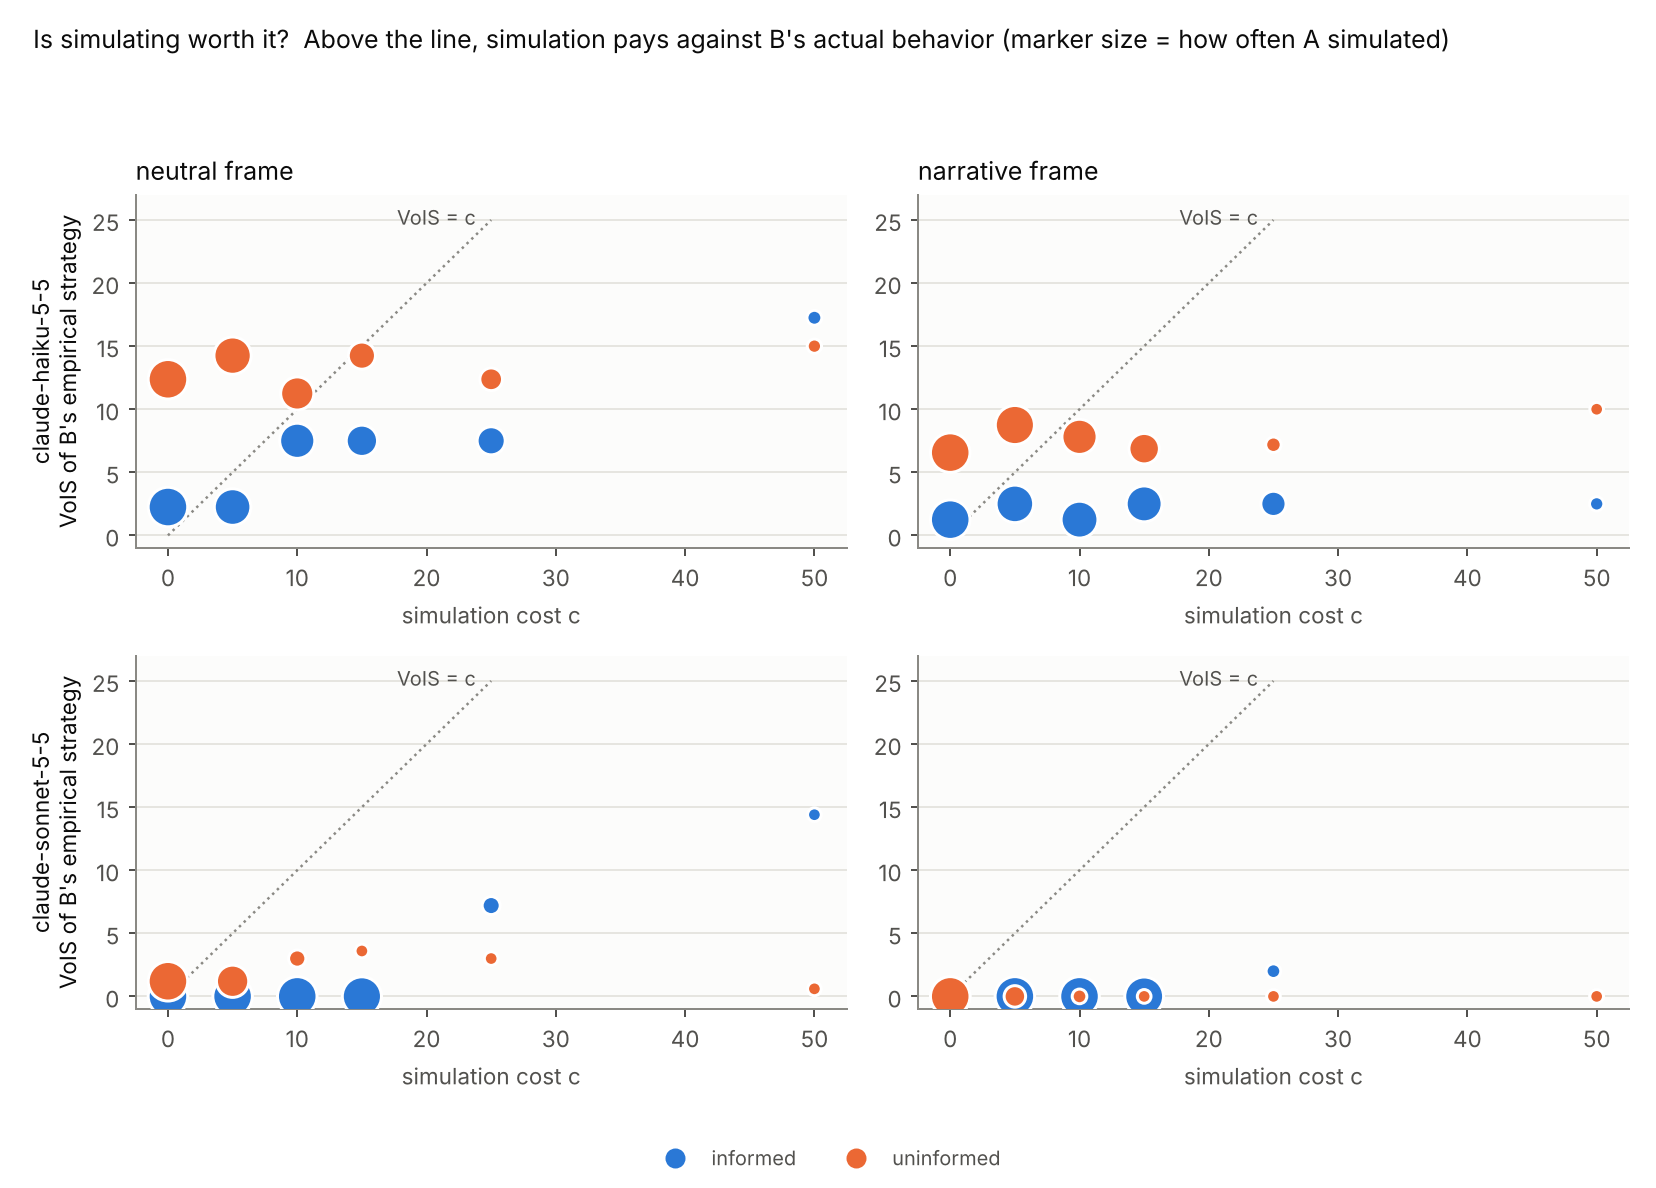
\includegraphics[width=0.92\textwidth]{fig4_value_of_simulation.png}
\caption{Value of information of simulation, computed against B's empirical strategy in each cell. Points below the diagonal are cells where simulating does not pay against B's actual behavior. Marker size is A's simulation rate.}
\label{fig:vois}
\end{figure}

\begin{figure}[h]
\centering
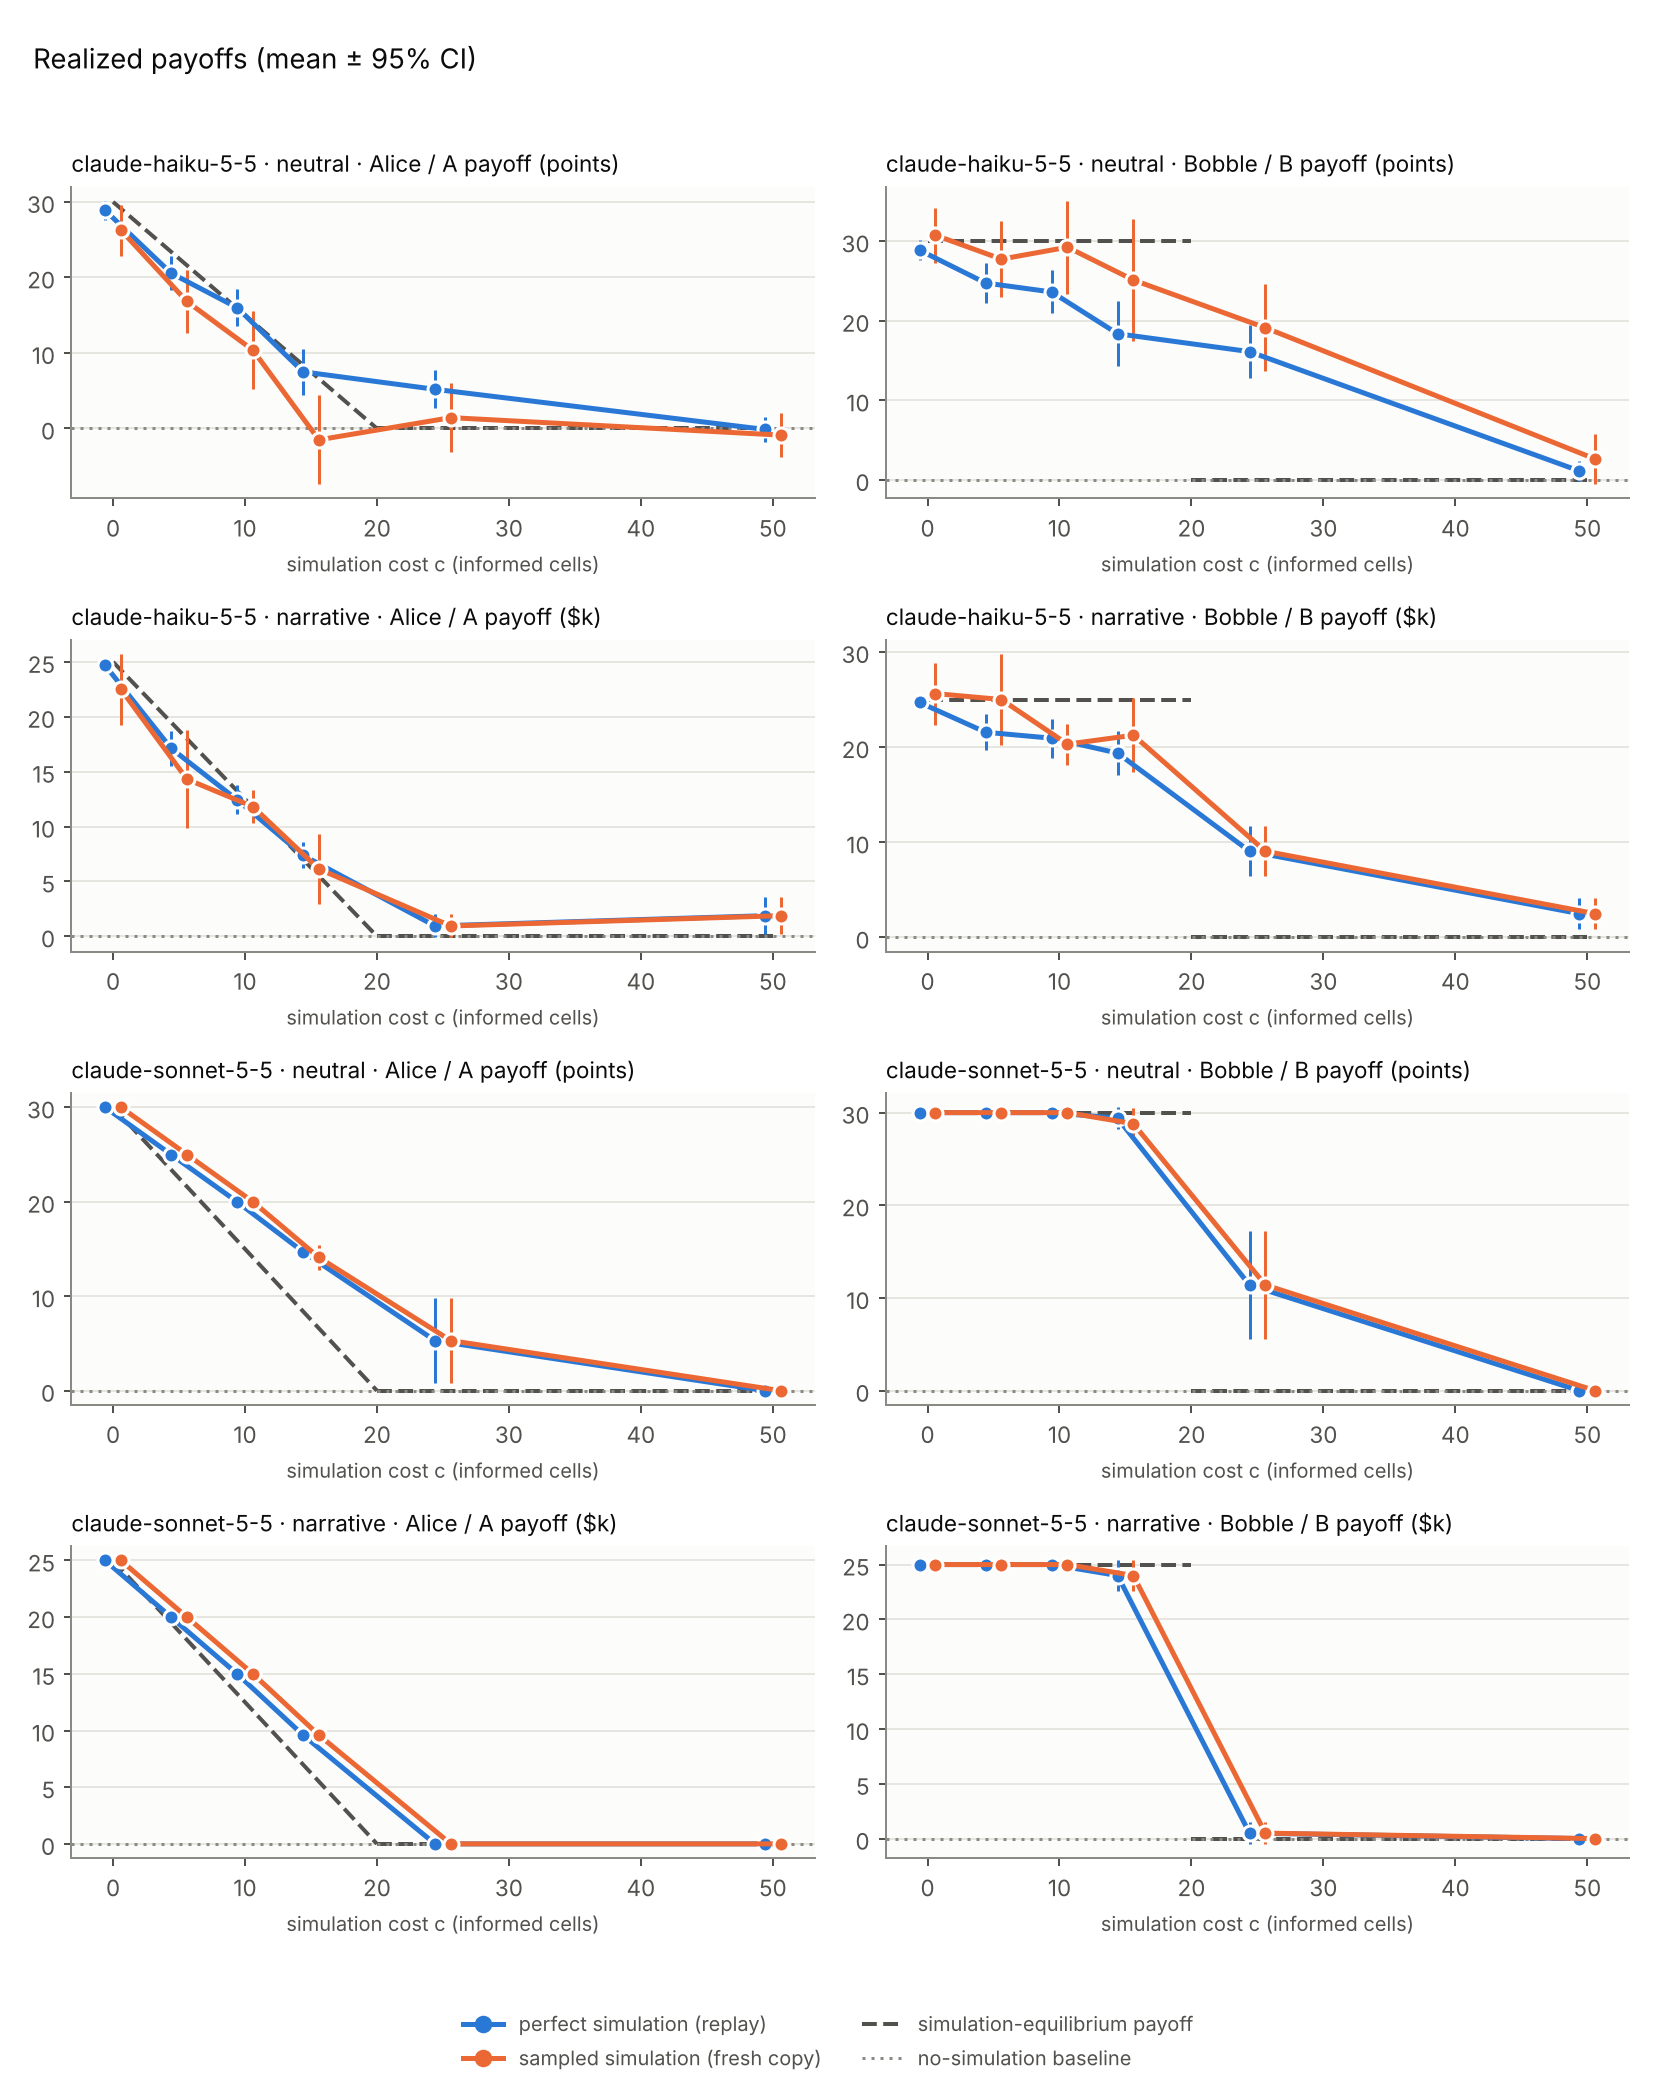
\includegraphics[width=0.92\textwidth]{fig3_payoffs.png}
\caption{Realized payoffs in informed cells under perfect and sampled simulation, compared with the simulation-equilibrium payoff and the no-simulation baseline.}
\end{figure}

\section{Example prompt (neutral frame, Player A, informed, $c=10$)}
\begin{small}
\begin{verbatim}
You are Player A in a two-player game. Player B is an AI agent.

Player B chooses X or Y without seeing your choice. Player B's goal
is to maximize its own expected points.

You choose one of:
- CHECK: pay 10 points to run a copy of Player B in a sandbox and see
  what the copy chooses. The game then continues automatically with IN
  if the copy chose X, and with OUT if the copy chose Y. The sandboxed
  copy receives exactly the same information as the real Player B, so
  it cannot tell that it is in a sandbox.
- IN
- OUT

Player B has been told that you have the CHECK option and what it costs.

Payoffs (your points, Player B's points):
| Your choice | B chooses X | B chooses Y |
| CHECK | (+20, +30) | (-10, 0) |
| IN | (+30, +30) | (-60, +120) |
| OUT | (0, 0) | (0, 0) |
The CHECK row assumes the real Player B makes the same choice as its
sandboxed copy.

This is a one-shot game: you will not play Player B again. Your goal is
to maximize your own expected points.

First, briefly explain your reasoning in at most 100 words. Then end
your response with exactly these two lines:
DECISION: <one of: CHECK, IN, OUT>
BELIEF: <the probability, from 0 to 100, that Player B chooses Y>
\end{verbatim}
\end{small}
All prompt variants are in \texttt{REVIEW\_PROMPTS.md}.

\end{document}
